\documentclass[11pt,a4paper]{article}

% -----------------------------------------------------------------------------
% Final technical report -- generated from final_technical_report.md
% Compile from latest/docs with: latexmk -pdf final_technical_report.tex
% -----------------------------------------------------------------------------
\usepackage[utf8]{inputenc}
\usepackage[T1]{fontenc}
\usepackage{lmodern}
\usepackage[a4paper,margin=22mm,headheight=15pt]{geometry}
\usepackage{microtype}
\usepackage{parskip}
\usepackage{setspace}
\usepackage{graphicx}
\graphicspath{{plots/}}
\usepackage{booktabs}
\usepackage{tabularx}
\usepackage{longtable}
\usepackage{array}
\usepackage{adjustbox}
\usepackage{multirow}
\usepackage{enumitem}
\usepackage{amsmath,amssymb}
\usepackage{xcolor}
\usepackage{tikz}
\usetikzlibrary{arrows.meta,backgrounds,calc,fit,positioning,shadows.blur,shapes.geometric,decorations.pathreplacing}
\usepackage[most]{tcolorbox}
\usepackage{listings}
\usepackage{caption}
\usepackage{subcaption}
\usepackage{float}
\usepackage{fancyhdr}
\usepackage{titlesec}
\usepackage{hyperref}
\usepackage[nameinlink,noabbrev]{cleveref}

\definecolor{navy}{HTML}{17365D}
\definecolor{ink}{HTML}{182230}
\definecolor{muted}{HTML}{607086}
\definecolor{inputblue}{HTML}{97ECF8}
\definecolor{processorange}{HTML}{FFD0AC}
\definecolor{rejectred}{HTML}{FFA0A0}
\definecolor{decisionyellow}{HTML}{FFF17B}
\definecolor{losspurple}{HTML}{ACA7FF}
\definecolor{traingreen}{HTML}{A4FFA1}
\definecolor{trainablepink}{HTML}{F4C5FF}
\definecolor{frozen}{HTML}{E0E0E0}
\definecolor{accent}{HTML}{1677C8}
\definecolor{deepgreen}{HTML}{16875D}
\definecolor{softbg}{HTML}{F5F8FC}

\hypersetup{
  colorlinks=true,
  linkcolor=navy,
  citecolor=deepgreen,
  urlcolor=accent,
  pdftitle={Occlusion-Robust Face Identification with a Partially Fine-Tuned ArcFace Model},
  pdfauthor={CSE 4112 Machine Learning Laboratory, KUET}
}

\pagestyle{fancy}
\fancyhf{}
\lhead{Occlusion-Robust Face Identification}
\rhead{Technical Report}
\cfoot{\thepage}
\renewcommand{\headrulewidth}{0.35pt}
\setlength{\emergencystretch}{2em}
\setcounter{tocdepth}{2}
\setcounter{secnumdepth}{3}
\titleformat{\section}{\Large\bfseries\color{navy}}{\thesection}{0.7em}{}
\titleformat{\subsection}{\large\bfseries\color{ink}}{\thesubsection}{0.7em}{}
\captionsetup{font=small,labelfont={bf,color=navy},justification=centering}

\newcommand{\code}[1]{\texttt{#1}}
\newcommand{\pct}{\%}
\newcommand{\good}[1]{\textbf{\color{deepgreen}#1}}
\newcommand{\bad}[1]{\textbf{\color{red!70!black}#1}}
\newcommand{\plot}[3][0.94\linewidth]{%
  \begin{figure}[H]\centering
    \includegraphics[width=#1,height=.74\textheight,keepaspectratio]{#2}
    \caption{#3}
  \end{figure}}

\tikzset{
  >={Latex[length=2.3mm,width=1.6mm]},
  flow/.style={-Latex,very thick,draw=navy!78,rounded corners=3pt},
  backflow/.style={-Latex,very thick,draw=red!70!black,rounded corners=3pt},
  dashflow/.style={-Latex,thick,dashed,draw=muted},
  base/.style={draw=navy!72,very thick,rounded corners=6pt,align=center,
               minimum height=11mm,inner sep=5pt,font=\small,
               blur shadow={shadow blur steps=5,shadow xshift=.6pt,shadow yshift=-.6pt,
                            shadow opacity=22}},
  input/.style={base,fill=inputblue},
  process/.style={base,fill=processorange},
  decision/.style={base,fill=decisionyellow},
  reject/.style={base,fill=rejectred},
  loss/.style={base,fill=losspurple},
  train/.style={base,fill=traingreen},
  trainable/.style={base,fill=trainablepink},
  frozen/.style={base,fill=frozen},
  feature/.style={circle,draw=navy!75,very thick,minimum size=8mm,inner sep=0pt,
                  font=\scriptsize\bfseries,blur shadow={shadow blur steps=4,shadow opacity=18}},
  group/.style={draw=navy!45,dashed,rounded corners=9pt,inner sep=7pt,fill=white,fill opacity=.55},
  tag/.style={rounded corners=3pt,inner xsep=4pt,inner ysep=2pt,font=\scriptsize\bfseries,text=white}
}

\lstdefinestyle{reportcode}{
  basicstyle=\ttfamily\footnotesize,
  backgroundcolor=\color{softbg},
  frame=single,
  rulecolor=\color{navy!25},
  breaklines=true,
  columns=fullflexible,
  keepspaces=true,
  showstringspaces=false,
  xleftmargin=4pt,
  framexleftmargin=4pt
}
\lstset{style=reportcode}

\begin{document}
\hypersetup{pageanchor=false}
\pagenumbering{gobble}

\begin{titlepage}
  \centering
  \vspace*{16mm}
  {\Large\bfseries\color{navy} CSE 4112 Machine Learning Laboratory\par}
  \vspace{4mm}
  {\large Khulna University of Engineering \& Technology (KUET)\par}
  \vspace{24mm}
  \begin{tcolorbox}[width=.92\textwidth,colback=softbg,colframe=navy,
    arc=5mm,boxrule=1.2pt,left=8mm,right=8mm,top=10mm,bottom=10mm,
    enhanced,drop fuzzy shadow]
    \centering
    {\Huge\bfseries\color{navy} Occlusion-Robust\\[2mm] Face Identification\par}
    \vspace{5mm}
    {\LARGE with a Partially Fine-Tuned ArcFace Model\par}
  \end{tcolorbox}
  \vspace{18mm}
  {\Large Final Technical Report\par}
  \vspace{7mm}
  {\large Person-disjoint six-fold evaluation of E0, E1 and E2\par}
  \vfill
  \begin{tabular}{rl}
    \textbf{Dataset:} & 30 identities, 8 occlusion conditions, 5,988 aligned crops\\
    \textbf{Models:} & ArcFace IResNet-50 and SCRFD/RetinaFace\\
    \textbf{Random seed:} & 42\\
    \textbf{Report date:} & \today
  \end{tabular}
  \vspace{12mm}
\end{titlepage}

\clearpage
\hypersetup{pageanchor=true}
\pagenumbering{roman}
\tableofcontents
\clearpage
\listoffigures
\clearpage

\section*{Diagram legend}
\addcontentsline{toc}{section}{Diagram legend}
The following palette is used consistently in every architecture and workflow diagram.

\begin{center}
\renewcommand{\arraystretch}{1.35}
\begin{tabularx}{.92\linewidth}{>{\centering\arraybackslash}p{18mm}X}
\toprule
\textbf{Colour} & \textbf{Meaning}\\
\midrule
\tikz\node[rounded corners=2pt,fill=frozen,draw=navy!65,minimum width=13mm,minimum height=5mm] {}; & Frozen or inactive component\\
\tikz\node[rounded corners=2pt,fill=inputblue,draw=navy!65,minimum width=13mm,minimum height=5mm] {}; & Input or raw data\\
\tikz\node[rounded corners=2pt,fill=processorange,draw=navy!65,minimum width=13mm,minimum height=5mm] {}; & Processing or transform step\\
\tikz\node[rounded corners=2pt,fill=rejectred,draw=navy!65,minimum width=13mm,minimum height=5mm] {}; & Test split, held-out sample, or rejected result\\
\tikz\node[rounded corners=2pt,fill=decisionyellow,draw=navy!65,minimum width=13mm,minimum height=5mm] {}; & Validation split or decision point\\
\tikz\node[rounded corners=2pt,fill=losspurple,draw=navy!65,minimum width=13mm,minimum height=5mm] {}; & Loss, optimizer, or gradient flow\\
\tikz\node[rounded corners=2pt,fill=traingreen,draw=navy!65,minimum width=13mm,minimum height=5mm] {}; & Train split, accepted result, or correct result\\
\tikz\node[rounded corners=2pt,fill=trainablepink,draw=navy!65,minimum width=13mm,minimum height=5mm] {}; & Benchmark, gallery item, or trainable layer\\
\bottomrule
\end{tabularx}
\end{center}

\clearpage
\pagenumbering{arabic}

\section{Introduction and objective}

Face recognition systems degrade under real-world occlusion because commodity pretrained recognizers such as ArcFace are trained predominantly on unoccluded faces. This project asks two questions for a small, 30-person enrollment-style identification system:

\begin{enumerate}[leftmargin=*,itemsep=2pt]
  \item How much does a strong pretrained ArcFace backbone (\code{buffalo\_l}, IResNet-50) already tolerate occlusion without fine-tuning?
  \item Does partial fine-tuning on occluded photographs of one set of people transfer to identities never seen during fine-tuning, or does it merely memorize the training people?
\end{enumerate}

Three configurations are evaluated under the same protocol.

\begin{table}[H]
\centering
\caption{Experimental configurations.}
\begin{tabular}{lll}
\toprule
\textbf{Experiment} & \textbf{Backbone layers unfrozen} & \textbf{Trainable parameters}\\
\midrule
E0 & None; frozen pretrained backbone & 0\\
E1 & Last residual block only & 4,720,640\\
E2 & Last residual block and embedding head & 17,568,256\\
\bottomrule
\end{tabular}
\end{table}

Every configuration is tested with person-disjoint six-fold cross-validation. E1 and E2 are fine-tuned on 20 people and evaluated on five different people, rotating the roles so that all 30 people are tested exactly once. A match counts as correct only when it identifies the right person and its cosine similarity is at least 0.3, matching the accept/reject behaviour of an enrollment system with an \textsc{unknown} cutoff.

\section{Dataset}

\subsection{Collection and composition}

The dataset contains 30 people photographed under eight occlusion conditions, indoors, at regular and low illumination, using a phone camera. RetinaFace detection was applied to every photograph. Only images for which a face was detected enter \code{manifest.csv}, producing 5,988 aligned crops. A small number of raw images failed detection because the face was out of frame, too dark, or too severely occluded.

\begin{figure}[H]
\centering
\begin{subfigure}{.49\linewidth}\centering
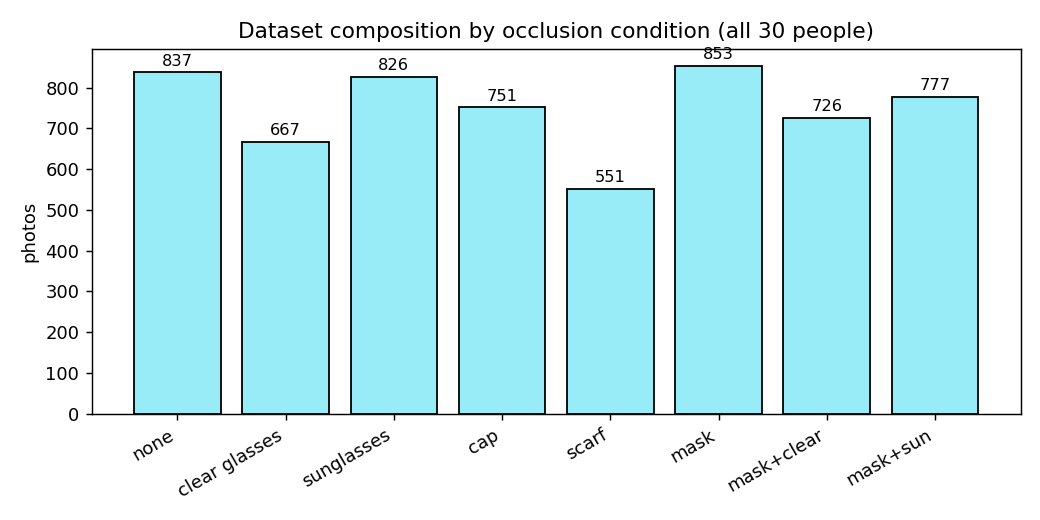
\includegraphics[width=\linewidth]{dataset_occlusion_counts.png}
\caption{Images by occlusion condition.}
\end{subfigure}\hfill
\begin{subfigure}{.49\linewidth}\centering
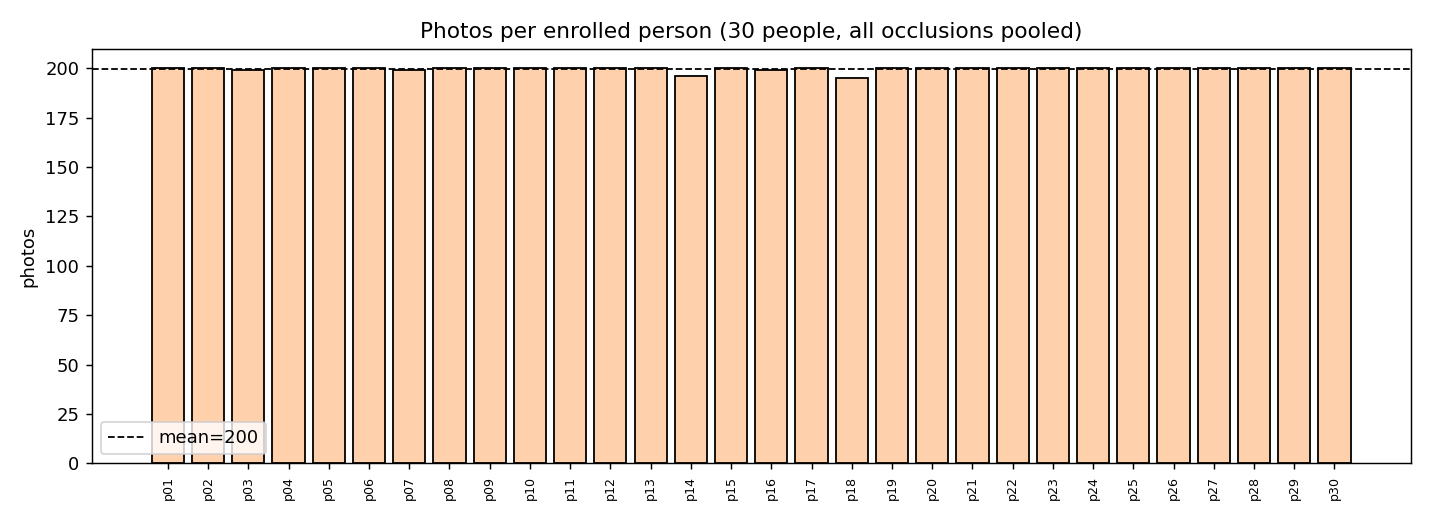
\includegraphics[width=\linewidth]{dataset_person_counts.png}
\caption{Images per person.}
\end{subfigure}
\caption{Dataset composition after face detection and alignment.}
\end{figure}

Coverage is not perfectly uniform. Two people are missing one occlusion condition each, and \code{scarf} has fewer photographs because it was added to the protocol later: only 24 of 30 people have that condition. Consequently, its per-occlusion result is based on a smaller and less diverse sample.

\subsection{Detection and alignment pipeline}

Every raw photograph passes through the same two-stage preprocessing pipeline before ArcFace receives it.

\begin{figure}[H]
\centering
\resizebox{\linewidth}{!}{%
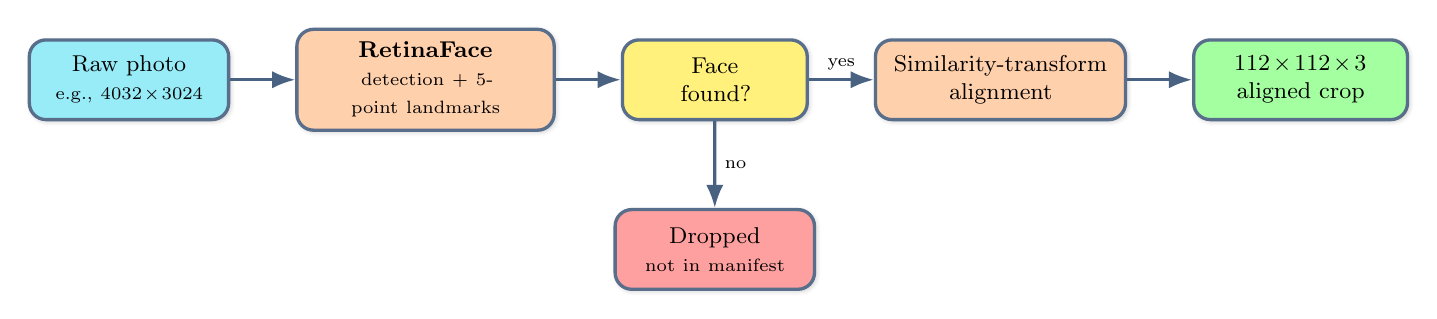
\begin{tikzpicture}[node distance=7mm and 9mm,scale=.92,transform shape]
  \node[input,text width=24mm] (raw) {Raw photo\\\scriptsize e.g., $4032\!\times\!3024$};
  \node[process,text width=32mm,right=of raw] (det) {\textbf{RetinaFace}\\\scriptsize detection + 5-point landmarks};
  \node[decision,text width=22mm,right=of det] (found) {Face\\found?};
  \node[process,text width=31mm,right=of found] (align) {Similarity-transform\\alignment};
  \node[train,text width=26mm,right=of align] (crop) {$112\!\times\!112\!\times\!3$\\aligned crop};
  \node[reject,text width=24mm,below=12mm of found] (drop) {Dropped\\\scriptsize not in manifest};
  \draw[flow] (raw)--(det);
  \draw[flow] (det)--(found);
  \draw[flow] (found)--node[above,font=\scriptsize]{yes}(align);
  \draw[flow] (align)--(crop);
  \draw[flow] (found)--node[right,font=\scriptsize]{no}(drop);
\end{tikzpicture}
}
\caption{Face detection and canonical alignment pipeline. Rounded colour-coded stages are used throughout the report.}
\label{fig:preprocess}
\end{figure}

For each crop, \code{manifest.csv} stores \code{person\_id}, \code{occlusion}, \code{lighting}, the RetinaFace detection confidence \code{det\_score}, and \code{bbox\_area\_frac}. Detector confidence is not uniform: occluded faces are systematically harder to detect, not merely harder to recognize.

\plot{dataset_det_score_hist.png}{Distribution of RetinaFace detection confidence over retained images.}

\subsection{Sample data}

\begin{figure}[H]
\centering
\begin{subfigure}{\linewidth}\centering
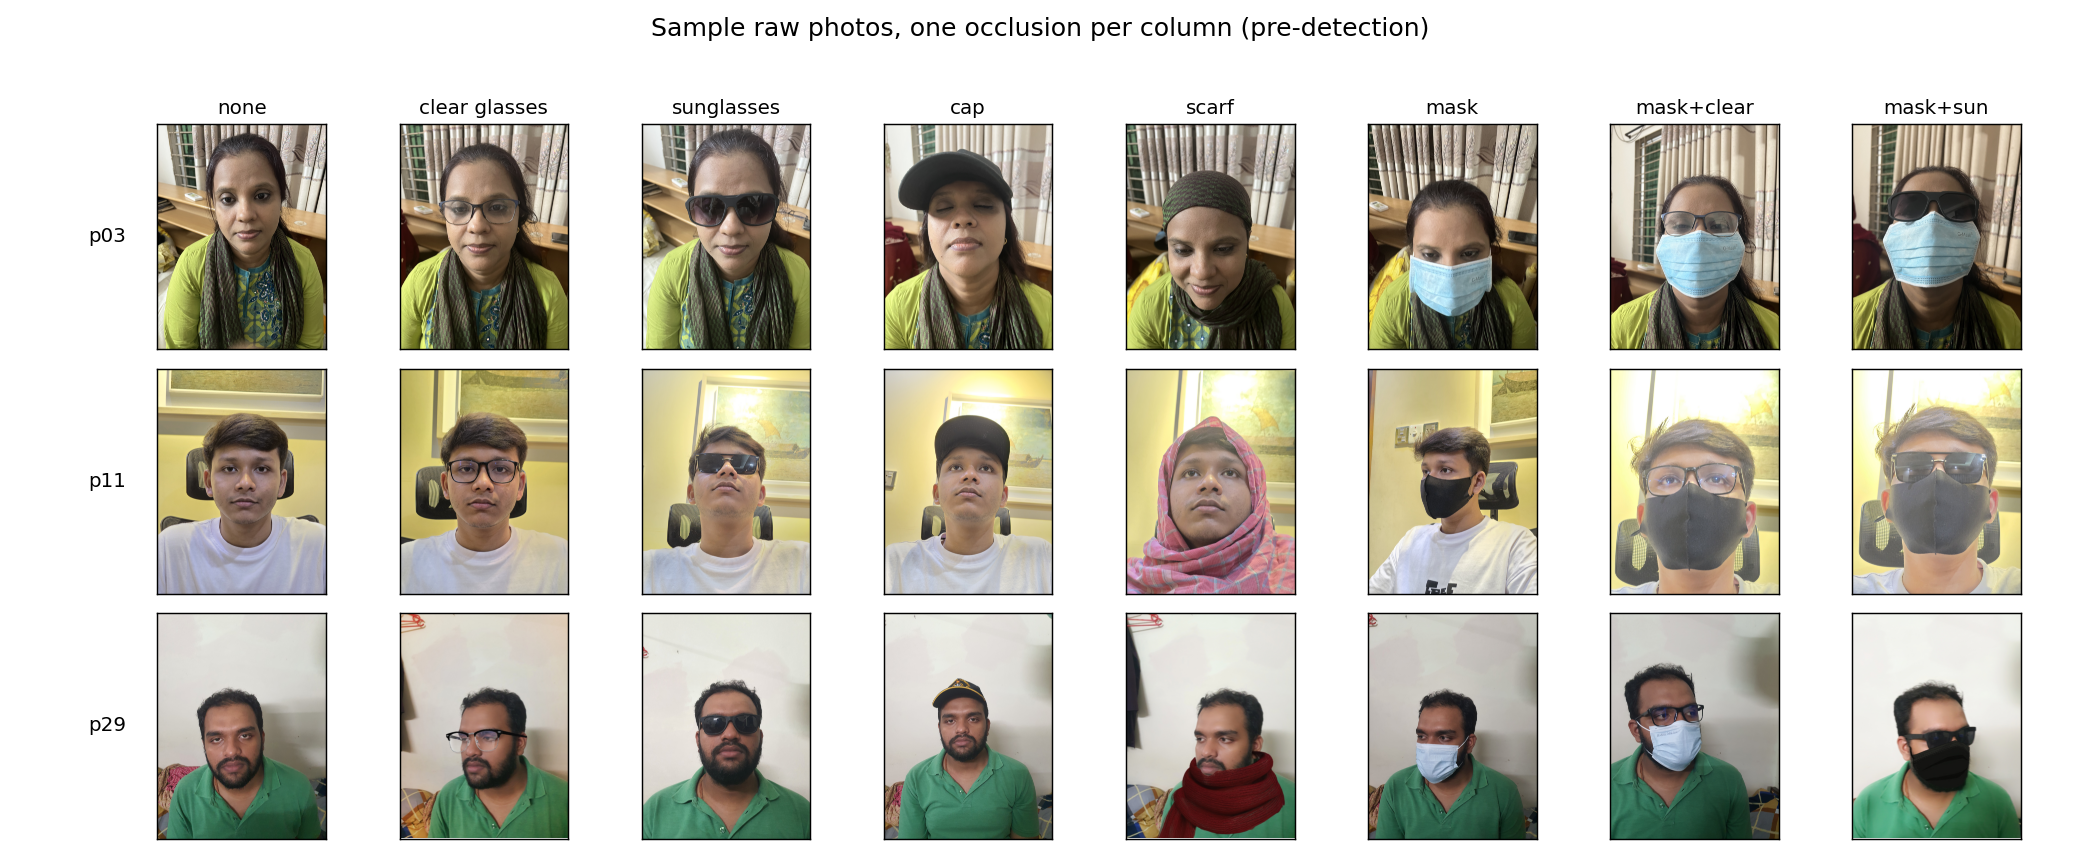
\includegraphics[width=.96\linewidth]{sample_raw_grid.png}
\caption{Raw phone-camera photographs.}
\end{subfigure}
\vspace{3mm}
\begin{subfigure}{\linewidth}\centering
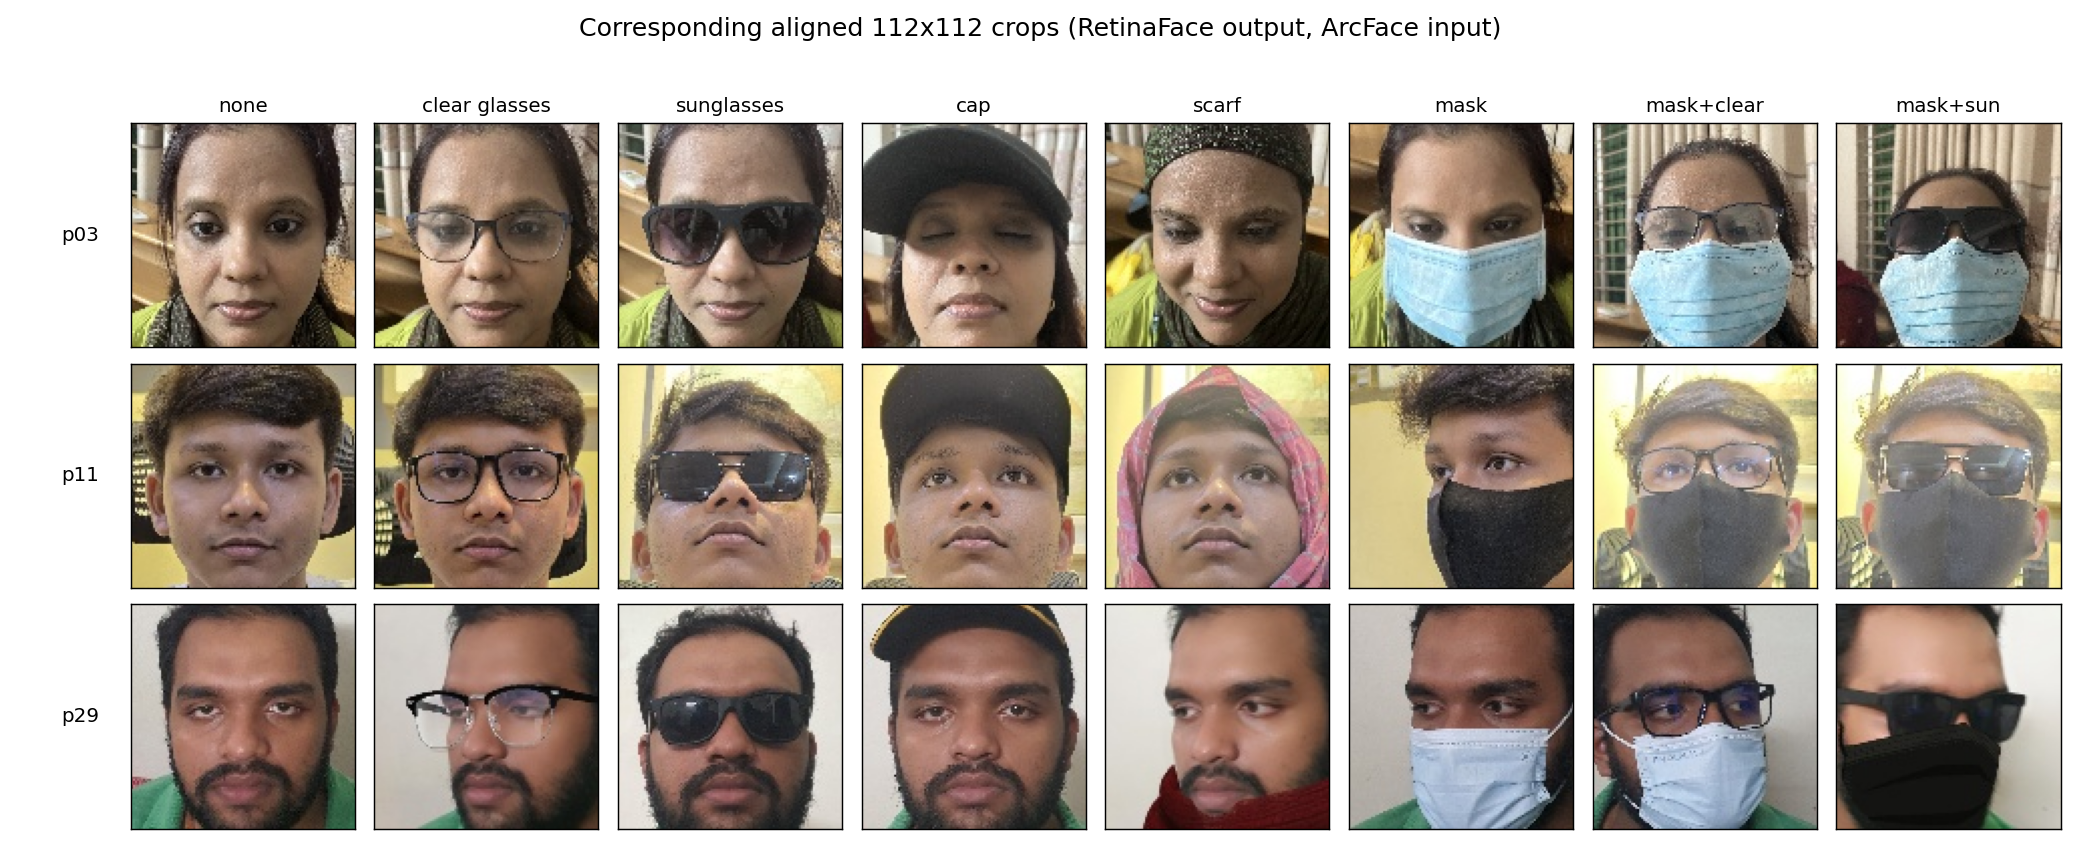
\includegraphics[width=.96\linewidth]{sample_crops_grid.png}
\caption{The corresponding aligned crops received by ArcFace.}
\end{subfigure}
\caption{Representative people across the eight occlusion conditions.}
\end{figure}

\subsection{RetinaFace failure cases}

Twelve of 6,000 raw photographs (0.2\pct) contain no face that RetinaFace could detect. These images never enter \code{manifest.csv} and are therefore absent from all E0/E1/E2 experiments. They were recovered by comparing all raw files against \code{manifest.csv} in \code{scripts/24\_report\_figures.py}.

\plot{retinaface_failure_gallery.png}{All twelve RetinaFace detection failures.}

Five photographs of person \code{p18} use a steep downward camera angle and combine extreme pitch with \code{mask\_sunglass} occlusion. The remaining seven images (\code{p03}, \code{p07}, four from \code{p14}, and \code{p16}) combine a mask or mask--sunglasses with severe underexposure. Every detection failure occurs under \code{mask}, \code{mask\_sunglass}, or extreme pose and lighting. Thus, the identification results are conditioned on detection having succeeded; true end-to-end performance on the hardest condition is slightly worse than the reported recognition accuracy. Two additional raw files are DNG captures that were never converted to JPEG; this is a format-handling issue and is not counted as a detection failure.

\section{Data splitting strategy}

\subsection{Why a person-disjoint split is necessary}

Generalization to unseen people can only be measured if no photograph of a test identity is visible during training. The dataset contains near-duplicate burst frames with a shared \code{group\_id}. An image-level random split can put almost identical frames of the same person on both sides of the split. The experiment therefore assigns complete identities, not individual images: all images of a person share the same role within a fold.

\subsection{Six-fold person-disjoint rotation}

The 30 people are shuffled once with seed 42 and partitioned into six blocks of five. Fold $k$ uses block $k$ as test, block $(k+1)\bmod 6$ as validation, and the remaining four blocks as training. Every person appears exactly once as test and once as validation.

\begin{figure}[H]
\centering
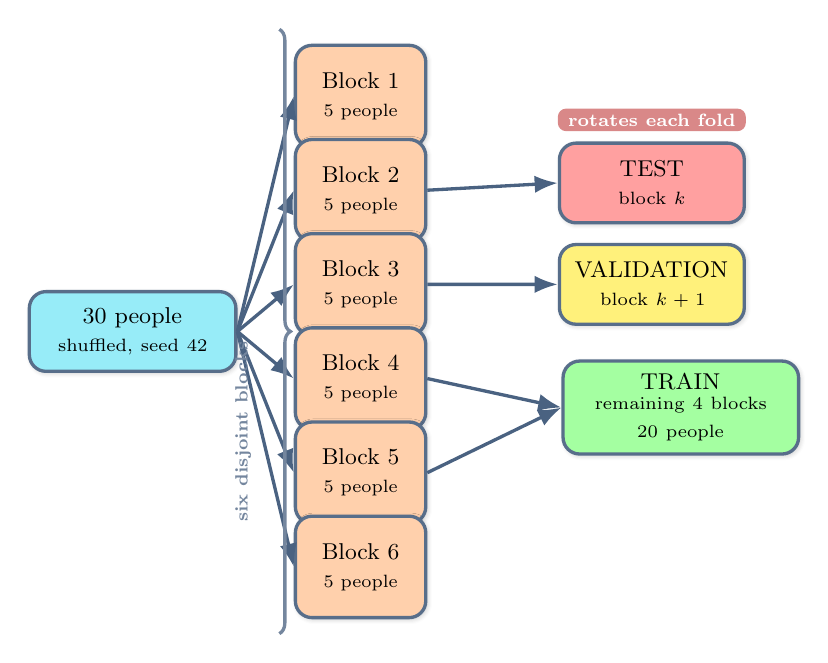
\begin{tikzpicture}[node distance=7mm and 7mm,scale=.92,transform shape]
  \node[input,text width=25mm] (all) {30 people\\\scriptsize shuffled, seed 42};
  \foreach \i in {1,...,6}{
    \node[process,minimum width=18mm,minimum height=14mm] (b\i) at ($(all.east)+(17mm,{(3.5-\i)*13mm})$) {Block \i\\\scriptsize 5 people};
  }
  \node[reject,text width=22mm] (test) at ($(b3.east)+(31mm,14mm)$) {TEST\\\scriptsize block $k$};
  \node[decision,text width=22mm] (val) at ($(b3.east)+(31mm,0)$) {VALIDATION\\\scriptsize block $k+1$};
  \node[train,text width=29mm] (trainset) at ($(b3.east)+(35mm,-17mm)$) {TRAIN\\\scriptsize remaining 4 blocks\\20 people};
  \foreach \i in {1,...,6}{\draw[flow] (all.east)--(b\i.west);}
  \draw[flow] (b2.east)--(test.west);
  \draw[flow] (b3.east)--(val.west);
  \draw[flow] (b4.east)--(trainset.west);
  \draw[flow] (b5.east)--(trainset.west);
  \node[tag,fill=rejectred!85!black] at ($(test.north)+(0,3mm)$) {rotates each fold};
  \draw[decorate,decoration={brace,amplitude=4pt},very thick,navy!60]
     ($(b1.north west)+(-2mm,2mm)$)--($(b6.south west)+(-2mm,-2mm)$)
     node[midway,left=5mm,rotate=90,font=\scriptsize\bfseries]{six disjoint blocks};
\end{tikzpicture}
\caption{Identity-level six-fold rotation. The arrows illustrate one fold; the roles rotate cyclically.}
\end{figure}

Fold 1 exactly reproduces the earlier single-fold version of the experiment. The full role assignment for all identities and folds is shown below.

\plot{fold_assignment_grid.png}{Train, validation, and test assignment of each identity across six folds.}

\subsection{Benchmark embedding selection}

Each person has exactly one clean gallery benchmark. It is selected only from that person's unoccluded (\code{none}) images, choosing the candidate with maximum RetinaFace confidence.

\begin{figure}[H]
\centering
\resizebox{\linewidth}{!}{%
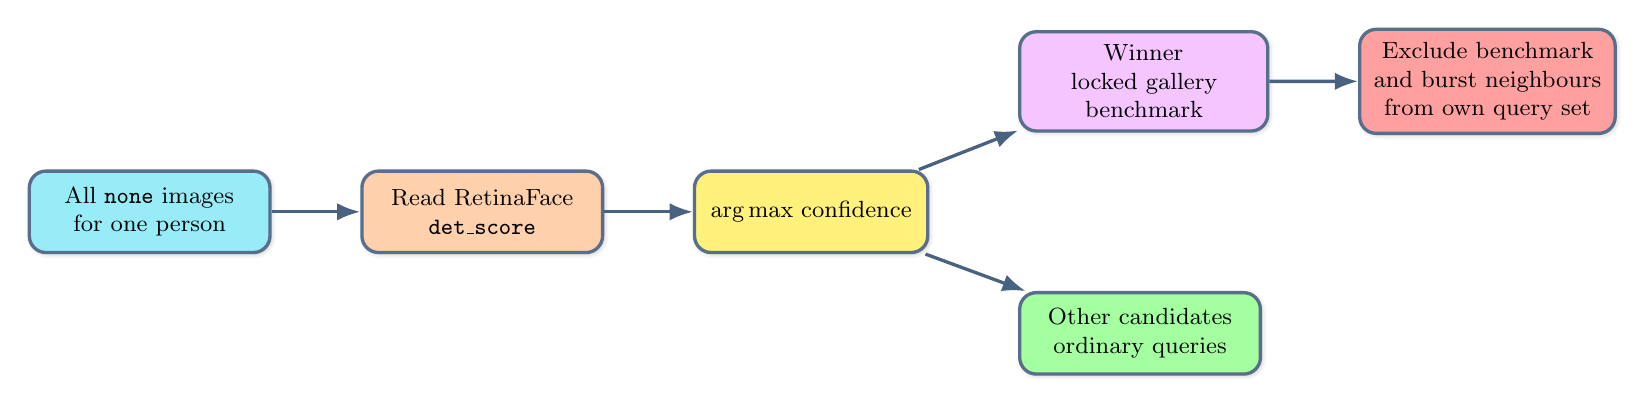
\begin{tikzpicture}[node distance=8mm and 12mm,scale=.94,transform shape]
  \node[input,text width=29mm] (none) {All \code{none} images\\for one person};
  \node[process,text width=29mm,right=of none] (scores) {Read RetinaFace\\\code{det\_score}};
  \node[decision,text width=28mm,right=of scores] (max) {$\arg\max$ confidence};
  \node[trainable,text width=30mm,above right=5mm and 12mm of max] (winner) {Winner\\locked gallery benchmark};
  \node[train,text width=29mm,below right=5mm and 12mm of max] (queries) {Other candidates\\ordinary queries};
  \node[reject,text width=31mm,right=of winner] (exclude) {Exclude benchmark\\and burst neighbours\\from own query set};
  \draw[flow] (none)--(scores); \draw[flow] (scores)--(max);
  \draw[flow] (max)--(winner); \draw[flow] (max)--(queries); \draw[flow] (winner)--(exclude);
\end{tikzpicture}
}
\caption{Selection and leakage-safe use of the benchmark embedding.}
\end{figure}

The benchmark and its near-duplicate burst frames are excluded from the person's query set. Selection is fold-independent: the same 30 embeddings in \code{runs/e1e2/person\_benchmarks.npz} are reused in every fold.

\plot{benchmark_selection_example.png}{Example selection for person p03; the outlined candidate becomes the benchmark.}

\subsection{Acceptance threshold}

A prediction is correct only when (1) the nearest of all 30 gallery benchmarks belongs to the query's true identity and (2) cosine similarity is at least 0.3. Below 0.3 the system returns \textsc{rejected}, even when the nearest identity happens to be correct. Because every test identity is enrolled in the gallery, a rejection is always a miss on a real person rather than a correct rejection of a stranger.

\section{Model architectures}

Both networks are \code{buffalo\_l} ONNX models from InsightFace, converted with \code{onnx2torch}. Numerical equivalence to ONNX Runtime is checked before fine-tuning, requiring cosine similarity of at least 0.999. Layer names, shapes, and parameter counts below were extracted from the actual ONNX graphs in \code{models/}.

\subsection{ArcFace recognizer: IResNet-50}

The recognizer \code{w600k\_r50.onnx} receives an RGB tensor of shape $[N,3,112,112]$, normalized as $(p-127.5)/127.5$, and emits one 512-dimensional embedding per face. It contains 43,590,976 parameters: a stem, four residual stages with $[3,4,14,3]$ blocks, and an embedding head.

\begin{figure}[H]
\centering
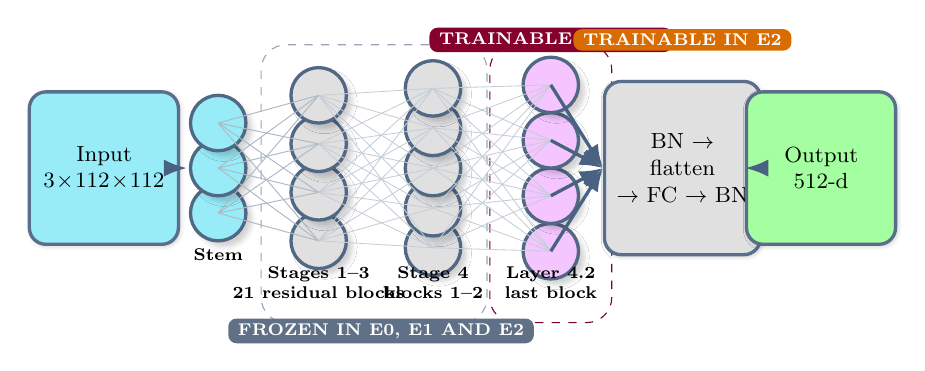
\begin{tikzpicture}[x=1cm,y=1cm,scale=.88,transform shape]
  % Layer groups
  \node[input,text width=18mm,minimum height=22mm] (img) at (0,0) {Input\\$3\!\times\!112\!\times\!112$};
  \foreach \y/\c in {-0.65/inputblue,0/inputblue,0.65/inputblue}
    \node[feature,fill=\c] at (1.65,\y) {};
  \node[font=\scriptsize\bfseries] at (1.65,-1.25) {Stem};
  \foreach \y in {-1.05,-.35,.35,1.05}
    \node[feature,fill=frozen] (s1\y) at (3.1,\y) {};
  \node[font=\scriptsize\bfseries,align=center] at (3.1,-1.65) {Stages 1--3\\21 residual blocks};
  \foreach \y in {-1.15,-.58,0,.58,1.15}
    \node[feature,fill=frozen] at (4.75,\y) {};
  \node[font=\scriptsize\bfseries,align=center] at (4.75,-1.65) {Stage 4\\blocks 1--2};
  \foreach \y in {-1.2,-.4,.4,1.2}
    \node[feature,fill=trainablepink] at (6.45,\y) {};
  \node[font=\scriptsize\bfseries,align=center] at (6.45,-1.65) {Layer 4.2\\last block};
  \node[frozen,text width=19mm,minimum height=25mm] (head) at (8.35,0) {BN $\to$ flatten\\$\to$ FC $\to$ BN};
  \node[train,text width=18mm,minimum height=22mm] (emb) at (10.35,0) {Output\\512-d};

  \draw[flow] (img)--(1.2,0);
  \foreach \a in {-0.65,0,0.65}{\foreach \b in {-1.05,-.35,.35,1.05}{\draw[navy!35,line width=.35pt] (1.65,\a)--(3.1,\b);}}
  \foreach \a in {-1.05,-.35,.35,1.05}{\foreach \b in {-1.15,-.58,0,.58,1.15}{\draw[navy!25,line width=.3pt] (3.1,\a)--(4.75,\b);}}
  \foreach \a in {-1.15,-.58,0,.58,1.15}{\foreach \b in {-1.2,-.4,.4,1.2}{\draw[navy!25,line width=.3pt] (4.75,\a)--(6.45,\b);}}
  \foreach \a in {-1.2,-.4,.4,1.2}{\draw[flow] (6.45,\a)--(head.west);}
  \draw[flow] (head)--(emb);

  \node[tag,fill=muted] at (4,-2.35) {FROZEN IN E0, E1 AND E2};
  \node[tag,fill=purple!70!black] at (6.45,1.85) {TRAINABLE E1 + E2};
  \node[tag,fill=orange!85!black] at (8.35,1.85) {TRAINABLE IN E2};
  \begin{scope}[on background layer]
    \node[group,fit={(2.55,-1.95) (5.25,1.5)}] {};
    \node[group,draw=purple!65!black,fit={(5.85,-1.95) (7.05,1.5)}] {};
  \end{scope}
\end{tikzpicture}
\caption{ArcFace IResNet-50 as a neural-layer diagram. Circular banks represent successive feature groups; tags show the exact fine-tuning scope.}
\label{fig:arcface}
\end{figure}

E1 unfreezes only \code{layer4.2}: tensors \code{BatchNormalization\_121}, \code{Conv\_122}, and \code{Conv\_124}, totalling 4,720,640 trainable parameters. E2 additionally unfreezes \code{BatchNormalization\_126}, \code{Gemm\_128}, and \code{BatchNormalization\_129} in the embedding head, for 17,568,256 trainable parameters. The stem and earlier residual blocks remain frozen.

\subsection{RetinaFace-family detector: SCRFD}

The detector \code{det\_10g.onnx} is used only for detection and five-point landmark alignment. It is never fine-tuned and does not participate directly in E0/E1/E2 evaluation because those experiments use pre-aligned crops. The model accepts dynamic-resolution tensors $[1,3,H,W]$ and emits nine tensors: classification, bounding-box regression, and landmarks at each of three feature-pyramid levels.

\begin{table}[H]
\centering
\caption{SCRFD outputs for a $640\times640$ input.}
\begin{tabular}{cccccc}
\toprule
\textbf{Level} & \textbf{Stride} & \textbf{Map} & \textbf{Anchors} & \textbf{Score} & \textbf{BBox / landmark}\\
\midrule
P3 & 8  & $80\times80$ & 2/location & $[12800,1]$ & $[12800,4]$ / $[12800,10]$\\
P4 & 16 & $40\times40$ & 2/location & $[3200,1]$  & $[3200,4]$ / $[3200,10]$\\
P5 & 32 & $20\times20$ & 2/location & $[800,1]$   & $[800,4]$ / $[800,10]$\\
\bottomrule
\end{tabular}
\end{table}

It has 4,225,835 parameters and 158 ONNX nodes: 58 Conv, 36 ReLU, 16 Add, 3 AveragePool, 3 Sigmoid, 2 Resize, and 1 MaxPool.

\begin{figure}[H]
\centering
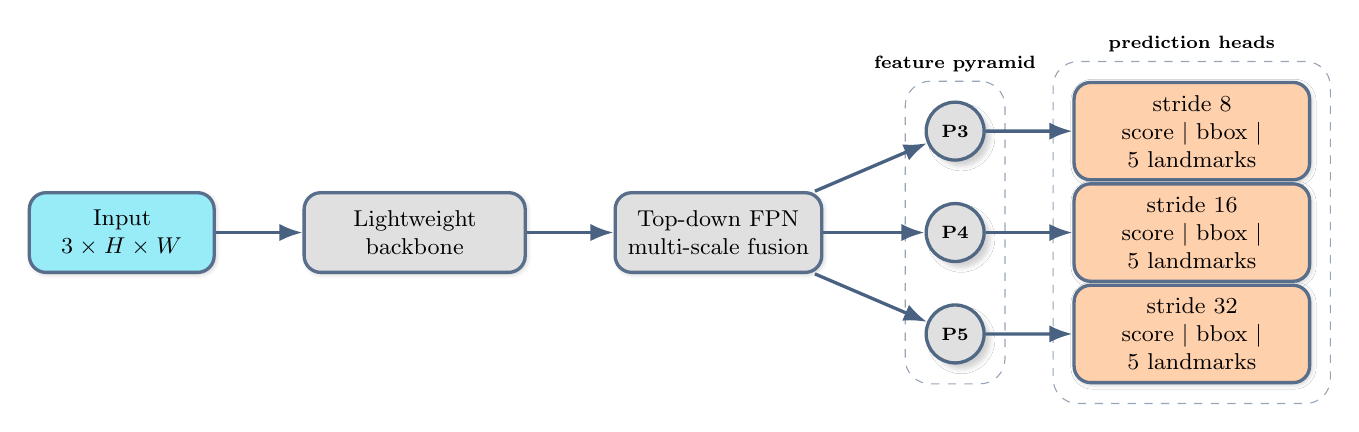
\begin{tikzpicture}[node distance=7mm and 12mm,scale=.92,transform shape]
  \node[input,text width=22mm] (in) {Input\\$3\times H\times W$};
  \node[frozen,text width=27mm,right=of in] (bb) {Lightweight\\backbone};
  \node[frozen,text width=25mm,right=of bb] (fpn) {Top-down FPN\\multi-scale fusion};
  \node[feature,fill=frozen,right=14mm of fpn,yshift=14mm] (p3) {P3};
  \node[feature,fill=frozen,right=14mm of fpn] (p4) {P4};
  \node[feature,fill=frozen,right=14mm of fpn,yshift=-14mm] (p5) {P5};
  \foreach \p/\lab in {p3/{stride 8},p4/{stride 16},p5/{stride 32}}{
    \node[process,text width=29mm,right=12mm of \p] (h\p) {\lab\\score $\mid$ bbox $\mid$\\5 landmarks};
    \draw[flow] (\p)--(h\p);
  }
  \draw[flow] (in)--(bb); \draw[flow] (bb)--(fpn);
  \draw[flow] (fpn)--(p3); \draw[flow] (fpn)--(p4); \draw[flow] (fpn)--(p5);
  \begin{scope}[on background layer]
    \node[group,fit=(p3)(p4)(p5),label={[font=\scriptsize\bfseries]above:feature pyramid}] {};
    \node[group,fit=(hp3)(hp4)(hp5),label={[font=\scriptsize\bfseries]above:prediction heads}] {};
  \end{scope}
\end{tikzpicture}
\caption{SCRFD multi-scale architecture. Each FPN feature level feeds three parallel prediction tasks.}
\end{figure}

\section{Experiments: E0, E1, and E2}

\subsection{Common protocol}

All experiments share the same data path, loss, and evaluation rule, differing only in which tensors have \code{requires\_grad=True}. Before training, the converted PyTorch graph is checked against ONNX Runtime on random input with required cosine similarity $\geq0.999$.

The classification ``head'' is not trainable. It consists of the 20 training people's L2-normalized benchmark embeddings, registered as a locked buffer. Each training image is pulled toward its own person's fixed direction and pushed away from the other 19 directions.

\begin{figure}[H]
\centering
\resizebox{\linewidth}{!}{%
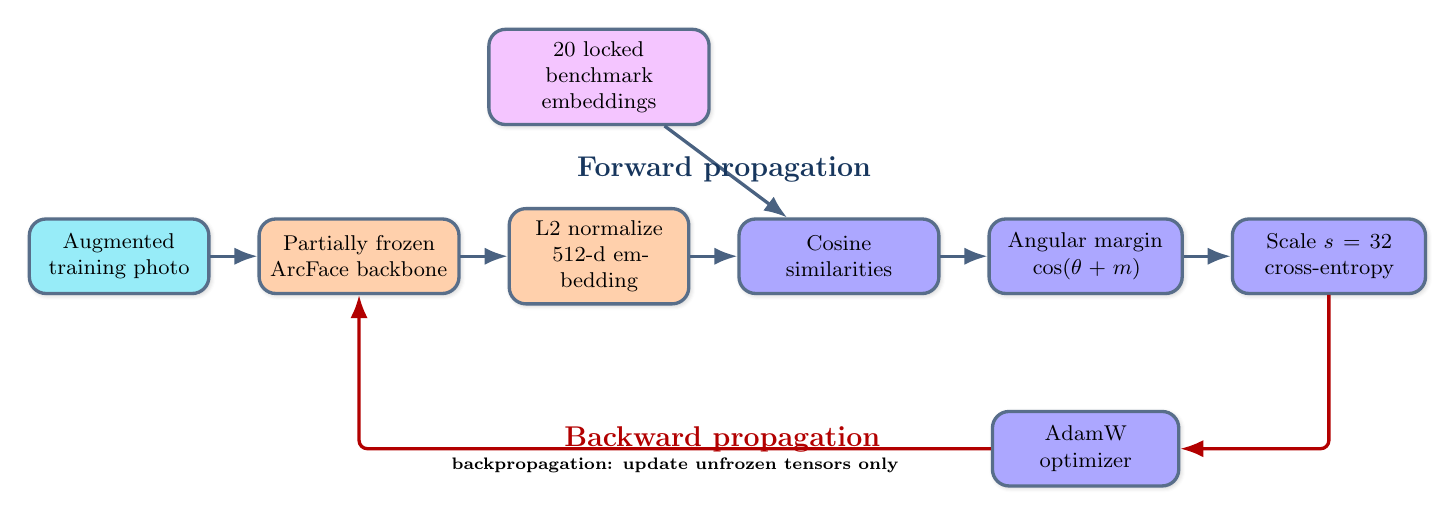
\begin{tikzpicture}[node distance=8mm and 7mm,scale=.86,transform shape]
  \node[input,text width=23mm] (x) {Augmented\\training photo};
  \node[process,text width=26mm,right=of x] (net) {Partially frozen\\ArcFace backbone};
  \node[process,text width=23mm,right=of net] (emb) {L2 normalize\\512-d embedding};
  \node[trainable,text width=29mm,above=12mm of emb] (gallery) {20 locked benchmark\\embeddings};
  \node[loss,text width=26mm,right=of emb] (cos) {Cosine\\similarities};
  \node[loss,text width=25mm,right=of cos] (margin) {Angular margin\\$\cos(\theta+m)$};
  \node[loss,text width=25mm,right=of margin] (ce) {Scale $s=32$\\cross-entropy};
  \node[loss,text width=24mm,below=17mm of margin] (opt) {AdamW\\optimizer};
  \draw[flow] (x)--(net); \draw[flow] (net)--(emb); \draw[flow] (emb)--(cos);
  \draw[flow] (gallery)--(cos); \draw[flow] (cos)--(margin); \draw[flow] (margin)--(ce);
  \draw[backflow] (ce.south)--(ce.south|-opt.east)--(opt.east);
  \draw[backflow] (opt.west)--node[below,font=\scriptsize\bfseries]{backpropagation: update unfrozen tensors only}(opt.west-|net.south)--(net.south);
  \node[above=4mm of $(x.north)!0.5!(ce.north)$,font=\large\bfseries,navy] {Forward propagation};
  \node[below=4mm of $(net.south)!0.5!(opt.south)$,font=\large\bfseries,red!70!black] {Backward propagation};
\end{tikzpicture}
}
\caption{Training computation graph, styled after a conventional forward/backward neural-network diagram.}
\label{fig:trainingloop}
\end{figure}

For the target class only, $\cos\theta$ is replaced by $\cos(\theta+m)$ before scaling. The margin is scheduled to avoid destabilizing the largely frozen backbone early in training.

\begin{figure}[H]
\centering
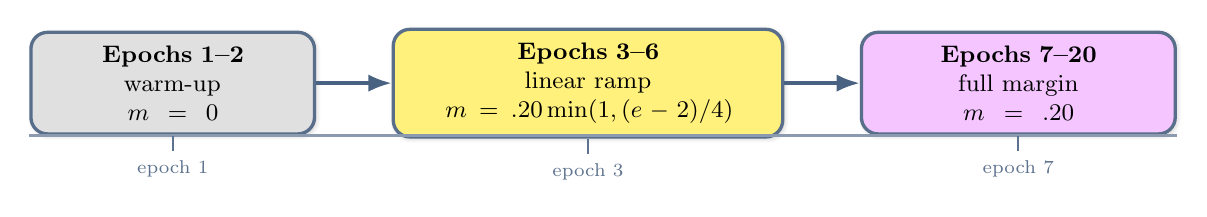
\begin{tikzpicture}[node distance=10mm,scale=.96,transform shape]
  \node[frozen,text width=34mm] (warm) {\textbf{Epochs 1--2}\\warm-up\\$m=0$};
  \node[decision,text width=48mm,right=of warm] (ramp) {\textbf{Epochs 3--6}\\linear ramp\\$m=.20\min(1,(e-2)/4)$};
  \node[trainable,text width=38mm,right=of ramp] (full) {\textbf{Epochs 7--20}\\full margin\\$m=.20$};
  \draw[flow] (warm)--(ramp); \draw[flow] (ramp)--(full);
  \draw[very thick,navy!50] (warm.south west)--(full.south east);
  \foreach \x/\lab in {warm/1,ramp/3,full/7}{\draw[navy!70,thick] (\x.south)--++(0,-2mm) node[below,font=\scriptsize]{epoch \lab};}
\end{tikzpicture}
\caption{ArcFace additive angular-margin schedule.}
\end{figure}

\begin{table}[H]
\centering
\caption{Training hyperparameters shared by E1 and E2.}
\begin{tabularx}{.88\linewidth}{>{\bfseries}lX}
\toprule
Hyperparameter & Value\\
\midrule
Optimizer & AdamW\\
Learning rate / weight decay & $3\times10^{-5}$ / $10^{-4}$\\
LR schedule & Cosine annealing, $T_{\max}=20$ epochs\\
Batch size & 32 training / 64 evaluation\\
Maximum epochs / patience & 20 / 5 epochs without improvement\\
ArcFace margin & 0.20; two warm-up epochs, then a four-epoch linear ramp\\
Loss scale / label smoothing & 32.0 / 0.1\\
Random seed & 42 for shuffle, folds, augmentation, and weight initialization\\
\bottomrule
\end{tabularx}
\end{table}

\paragraph{Frozen BatchNorm statistics.} \code{EmbeddingModel.train()} forces \code{self.backbone.eval()}. Running means and variances therefore remain fixed even when a BatchNorm layer's affine scale and bias are trainable. This stabilizes fine-tuning on only 20 identities and prevents the small, occlusion-skewed batches from replacing the pretrained statistics.

\paragraph{Light augmentation.} Training-only augmentation applies a horizontal flip ($p=.5$), downscale--upscale blur ($p=.3$), Gaussian blur ($p=.15$), Gaussian pixel noise ($p=.2$), JPEG recompression at quality 50--95 ($p=.3$), and brightness/contrast jitter ($p=.2$). The intent is capture-quality robustness rather than synthetic occlusion.

\paragraph{Selection and early stopping.} After each epoch, the model is scored on the fold's validation identities against the full 30-person gallery. The lexicographic key \code{(val\_acc, val\_gap)} is compared with strict \code{>}. Five consecutive non-improving epochs trigger early stopping. Epoch 0 is the pretrained baseline and initializes the best checkpoint; if training never beats it, the experiment retains the untrained model.

\subsection{E0: frozen baseline}

E0 unfreezes no parameters and runs with \code{--epochs 0}. It is the genuine pretrained \code{w600k\_r50.onnx} model, evaluated with the same gallery and 0.3 threshold as E1 and E2.

\subsection{E1: last residual block only}

E1 unfreezes \code{layer4.2}: \code{BatchNormalization\_121}, \code{Conv\_122}, and \code{Conv\_124}. These contain 4,720,640 parameters.

\begin{figure}[H]
\centering
\resizebox{\linewidth}{!}{%
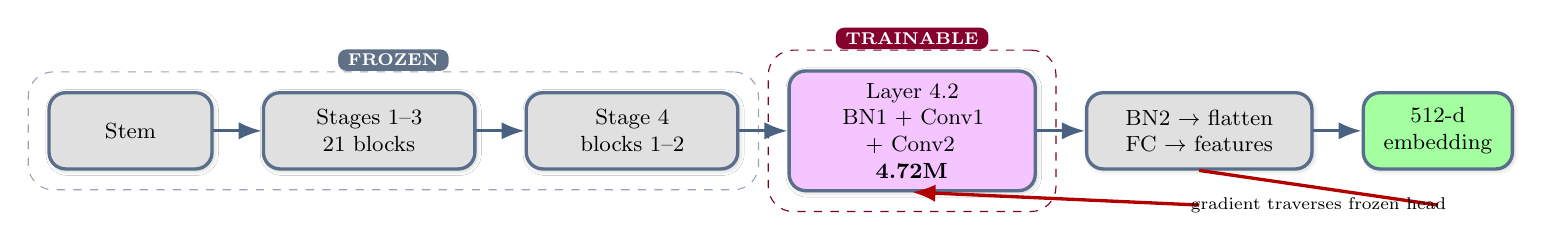
\begin{tikzpicture}[node distance=7mm,scale=.88,transform shape]
  \node[frozen,text width=20mm] (stem) {Stem};
  \node[frozen,text width=27mm,right=of stem] (s13) {Stages 1--3\\21 blocks};
  \node[frozen,text width=27mm,right=of s13] (s4) {Stage 4\\blocks 1--2};
  \node[trainable,text width=32mm,right=of s4] (last) {Layer 4.2\\BN1 + Conv1 + Conv2\\\textbf{4.72M}};
  \node[frozen,text width=29mm,right=of last] (head) {BN2 $\to$ flatten\\FC $\to$ features};
  \node[train,text width=18mm,right=of head] (out) {512-d\\embedding};
  \draw[flow] (stem)--(s13); \draw[flow] (s13)--(s4); \draw[flow] (s4)--(last);
  \draw[flow] (last)--(head); \draw[flow] (head)--(out);
  \draw[backflow] ($(out.south)+(0,-5mm)$)--node[below,font=\scriptsize]{gradient traverses frozen head}(head.south|-out.south)+(0,-5mm)--(last.south);
  \begin{scope}[on background layer]
    \node[group,fit=(stem)(s13)(s4),label={[tag,fill=muted]above:FROZEN}] {};
    \node[group,draw=purple!65!black,fit=(last),label={[tag,fill=purple!70!black]above:TRAINABLE}] {};
  \end{scope}
\end{tikzpicture}
}
\caption{E1 fine-tuning scope: only the last residual block is updated.}
\end{figure}

The chain rule still propagates gradients through the frozen embedding head to reach \code{layer4.2}, but the optimizer updates only that block. E1's selected epoch is 5 in five folds and 8 in fold 4, so the improvement generally appears quickly and then plateaus.

\subsection{E2: last residual block and embedding head}

E2 adds \code{BatchNormalization\_126}, \code{Gemm\_128}, and \code{BatchNormalization\_129} to the E1 scope. Its 17,568,256 trainable parameters are dominated by the $[512,25088]$ fully-connected matrix, which contains 12.85M parameters.

\begin{figure}[H]
\centering
\resizebox{\linewidth}{!}{%
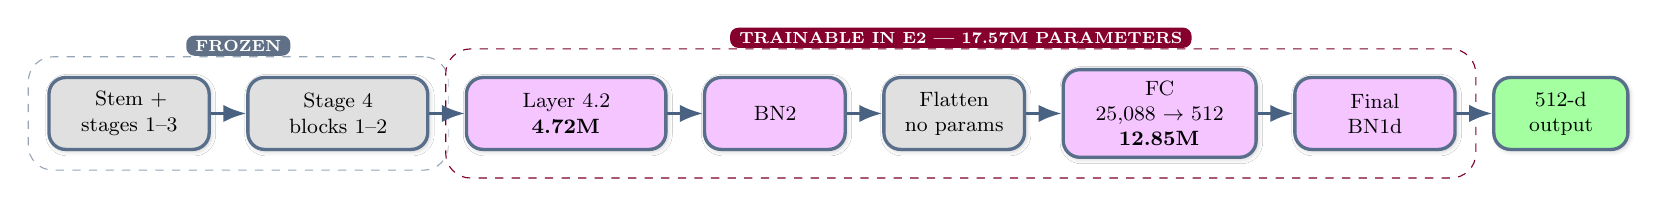
\begin{tikzpicture}[node distance=5.5mm,scale=.83,transform shape]
  \node[frozen,text width=21mm] (early) {Stem +\\stages 1--3};
  \node[frozen,text width=24mm,right=of early] (s4) {Stage 4\\blocks 1--2};
  \node[trainable,text width=27mm,right=of s4] (last) {Layer 4.2\\\textbf{4.72M}};
  \node[trainable,text width=18mm,right=of last] (bn) {BN2};
  \node[frozen,text width=18mm,right=of bn] (flat) {Flatten\\no params};
  \node[trainable,text width=26mm,right=of flat] (fc) {FC\\25,088 $\to$ 512\\\textbf{12.85M}};
  \node[trainable,text width=21mm,right=of fc] (feat) {Final\\BN1d};
  \node[train,text width=17mm,right=of feat] (out) {512-d\\output};
  \draw[flow] (early)--(s4); \draw[flow] (s4)--(last); \draw[flow] (last)--(bn);
  \draw[flow] (bn)--(flat); \draw[flow] (flat)--(fc); \draw[flow] (fc)--(feat); \draw[flow] (feat)--(out);
  \begin{scope}[on background layer]
    \node[group,fit=(early)(s4),label={[tag,fill=muted]above:FROZEN}] {};
    \node[group,draw=purple!65!black,fit=(last)(bn)(fc)(feat),label={[tag,fill=purple!70!black]above:TRAINABLE IN E2 --- 17.57M PARAMETERS}] {};
  \end{scope}
\end{tikzpicture}
}
\caption{E2 fine-tuning scope. The large FC projection can directly reshape the final embedding space.}
\end{figure}

E2 changes the coordinate system in which the loss is computed and has 3.7 times E1's trainable capacity. With only 20 training identities, it is more prone to identity-specific overfitting. In folds 3, 4, and 5, no E2 epoch beats epoch 0, so selection falls back to the pretrained checkpoint.

\section{Results}

All pooled values use exact per-fold counts rather than averaging percentages. The full evaluation contains 5,818 query images, and every identity is tested exactly once.

\subsection{Pooled accuracy and outcome types}

\begin{table}[H]
\centering
\caption{Pooled outcomes over 5,818 queries. Columns partition every query.}
\begin{adjustbox}{max width=\linewidth}
\begin{tabular}{lccccc}
\toprule
& \textbf{Accepted} & \textbf{Rejected: correct} & \textbf{Rejected: wrong} & \textbf{Misidentified} & \textbf{Beats E0}\\
& \textbf{and correct} & \textbf{top match $<.3$} & \textbf{top match $<.3$} & \textbf{wrong, $\geq.3$} & \textbf{by fold}\\
\midrule
E0 & 84.98\pct & 12.50\pct & 2.53\pct & 0.00\pct & ---\\
E1 & \good{86.18\pct} & 8.47\pct & 5.12\pct & 0.22\pct & \good{6/6}\\
E2 & 84.72\pct & 7.24\pct & 4.73\pct & \bad{3.32\pct} & 3/6\\
\bottomrule
\end{tabular}
\end{adjustbox}
\end{table}

The four outcome columns sum to the full sample for each row. An independent CPU reconstruction from the saved prediction files differs by only one image whose score lies within floating-point noise of 0.3; the table retains the original GPU results.

\plot{outcome_breakdown.png}{Pooled accepted, rejected, and misidentified outcomes.}

E1 is the only configuration that reliably improves on the pretrained model. It raises pooled accuracy by 1.20 percentage points, wins in every fold, and keeps confident wrong-person predictions to 0.22\pct. E2 is 0.26 points below E0 and converts more low-confidence rejections into confident errors: its 3.32\pct misidentification rate is materially less safe for an identification system.

\plot{arcface_failure_gallery.png}{Representative low-confidence ArcFace failures from E0.}

The top row still chooses the correct identity but with scores near 0.07--0.08, so the system rejects the result. The bottom row chooses the wrong nearest benchmark but also remains below 0.3, so these are rejections rather than misidentifications. All severe examples involve \code{mask\_sunglass}; E0 produces no confidently wrong result at the chosen threshold.

\subsection{Per-fold results}

\begin{table}[H]
\centering
\caption{Accuracy by held-out identity fold. Parentheses give the selected epoch.}
\begin{tabular}{clccc}
\toprule
\textbf{Fold} & \textbf{Test people} & \textbf{E0} & \textbf{E1} & \textbf{E2}\\
\midrule
1 & p11, p15, p20, p23, p27 & 84.39\pct & 86.76\pct (5) & 85.01\pct (5)\\
2 & p06, p07, p12, p13, p16 & 80.71\pct & 81.02\pct (5) & 81.02\pct (6)\\
3 & p10, p17, p22, p26, p30 & 88.60\pct & 89.02\pct (5) & 88.60\pct (\textbf{0})\\
4 & p02, p03, p14, p19, p28 & 80.47\pct & 82.01\pct (8) & 80.47\pct (\textbf{0})\\
5 & p05, p08, p18, p25, p29 & 90.83\pct & 92.40\pct (5) & 90.83\pct (\textbf{0})\\
6 & p01, p04, p09, p21, p24 & 85.02\pct & 86.06\pct (5) & 82.52\pct (6)\\
\bottomrule
\end{tabular}
\end{table}

Epoch 0 means that no training epoch improved on the frozen backbone. Full epoch-by-epoch histories are summarized below and preserved in \code{epoch\_curves.md}.

\plot{epoch_curves.png}{Training and validation histories for all folds and trainable configurations.}

\subsection{Per-occlusion performance}

\begin{table}[H]
\centering
\caption{Accuracy by occlusion condition.}
\begin{tabular}{lrrrr}
\toprule
\textbf{Occlusion} & \textbf{$n$} & \textbf{E0} & \textbf{E1} & \textbf{E2}\\
\midrule
none              & 667 & 100.0\pct & 99.4\pct & 99.6\pct\\
clearglass        & 667 & 100.0\pct & 99.0\pct & 98.7\pct\\
sunglass          & 826 & 98.5\pct  & 99.2\pct & 97.2\pct\\
scarf             & 551 & 97.3\pct  & 94.9\pct & 96.0\pct\\
cap               & 751 & 95.5\pct  & 95.2\pct & 94.3\pct\\
mask              & 853 & 90.2\pct  & 89.9\pct & 88.0\pct\\
mask\_clearglass & 726 & 68.5\pct  & 68.9\pct & 66.7\pct\\
\textbf{mask\_sunglass} & 777 & 35.6\pct & \good{47.2\pct} & 42.7\pct\\
\bottomrule
\end{tabular}
\end{table}

\plot{per_occlusion_accuracy.png}{Per-occlusion accuracy for E0, E1, and E2.}

The E1 improvement is concentrated almost entirely in \code{mask\_sunglass}, which hides both the lower face and eye region. Accuracy rises from 35.6\pct to 47.2\pct. Conditions that E0 already handles well remain flat or degrade slightly. E2 captures part of the hardest-condition gain but loses more accuracy elsewhere. The scarf result should be read with extra uncertainty because it represents only 24 identities.

\subsection{Learning curves}

The original training program computed validation accepted-correct rate, not validation loss. \code{scripts/25\_e1e2\_learning\_curve.py} reproduces training and adds a validation cross-entropy over the full 30-person gallery, using the cosine-similarity matrix already calculated during scoring. All original accuracy and selected-epoch values reproduce exactly.

\plot{learning_curve.png}{Training loss (solid) and validation loss (dashed) for every E1 and E2 fold.}

Both configurations show an epoch-1 loss spike as the first update perturbs the already useful pretrained embedding, followed by recovery. E1 settles into a comparatively tight band around epochs 5--6. E2 is higher and less consistent: fold 3 rises above 1.3, while fold 1 begins climbing again after epoch 6. This explains E2's fallback to epoch 0 in half of the folds and its less reliable test performance.

\subsection{Confusion matrices and macro metrics}

Each confusion matrix has 30 person columns plus \textsc{reject}. A sub-threshold query lowers recall for its true identity without lowering another person's precision.

\begin{table}[H]
\centering
\caption{Pooled macro metrics.}
\begin{tabular}{lrrrr}
\toprule
\textbf{Experiment} & \textbf{Accuracy} & \textbf{Macro precision} & \textbf{Macro recall} & \textbf{Macro F1}\\
\midrule
E0 & 84.98\pct & 100.00\pct & 85.12\pct & 91.67\pct\\
E1 & \good{86.18\pct} & 99.72\pct & \good{86.33\pct} & \good{92.15\pct}\\
E2 & 84.72\pct & 96.43\pct & 84.87\pct & 89.85\pct\\
\bottomrule
\end{tabular}
\end{table}

\begin{figure}[H]
\centering
\begin{subfigure}{.32\linewidth}\centering
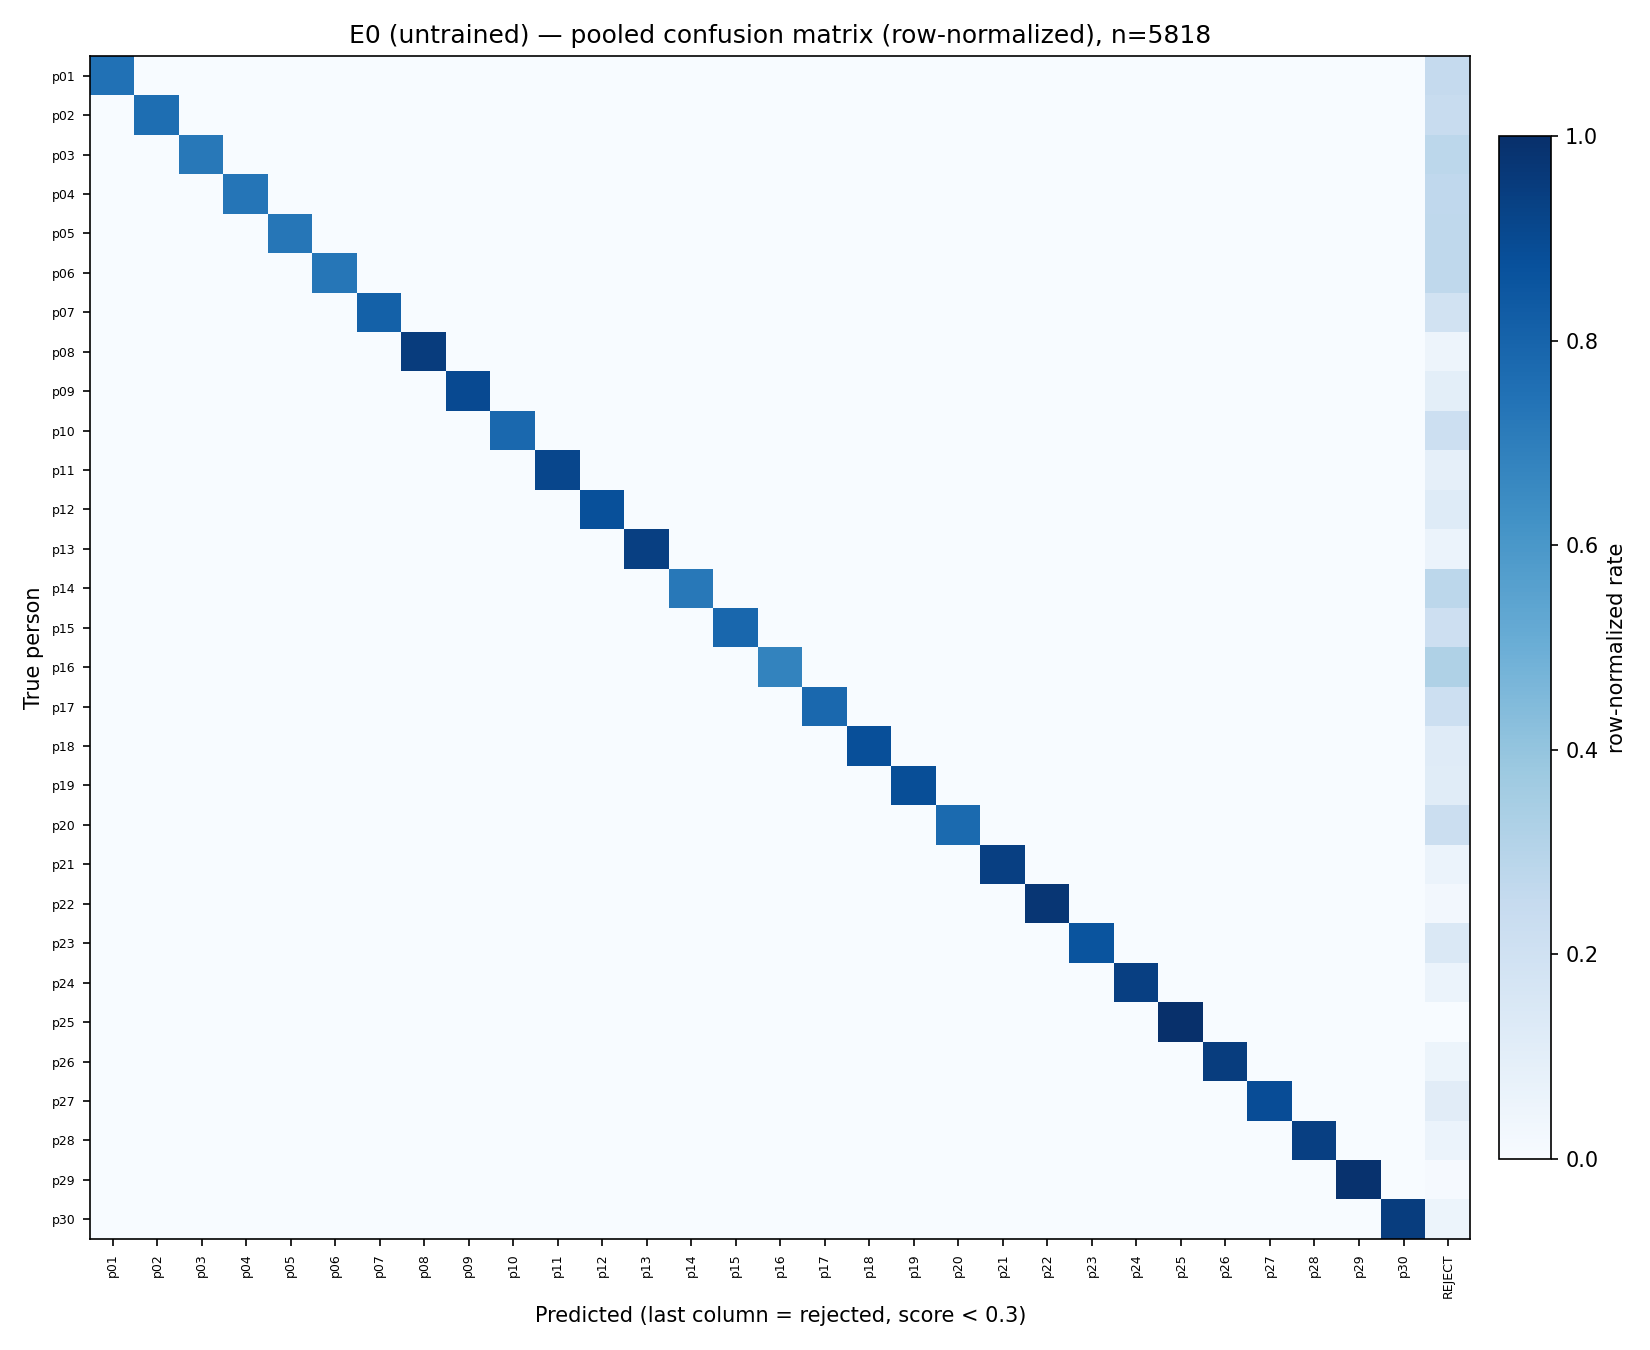
\includegraphics[width=\linewidth]{e0_confusion_overall.png}\caption{E0}
\end{subfigure}\hfill
\begin{subfigure}{.32\linewidth}\centering
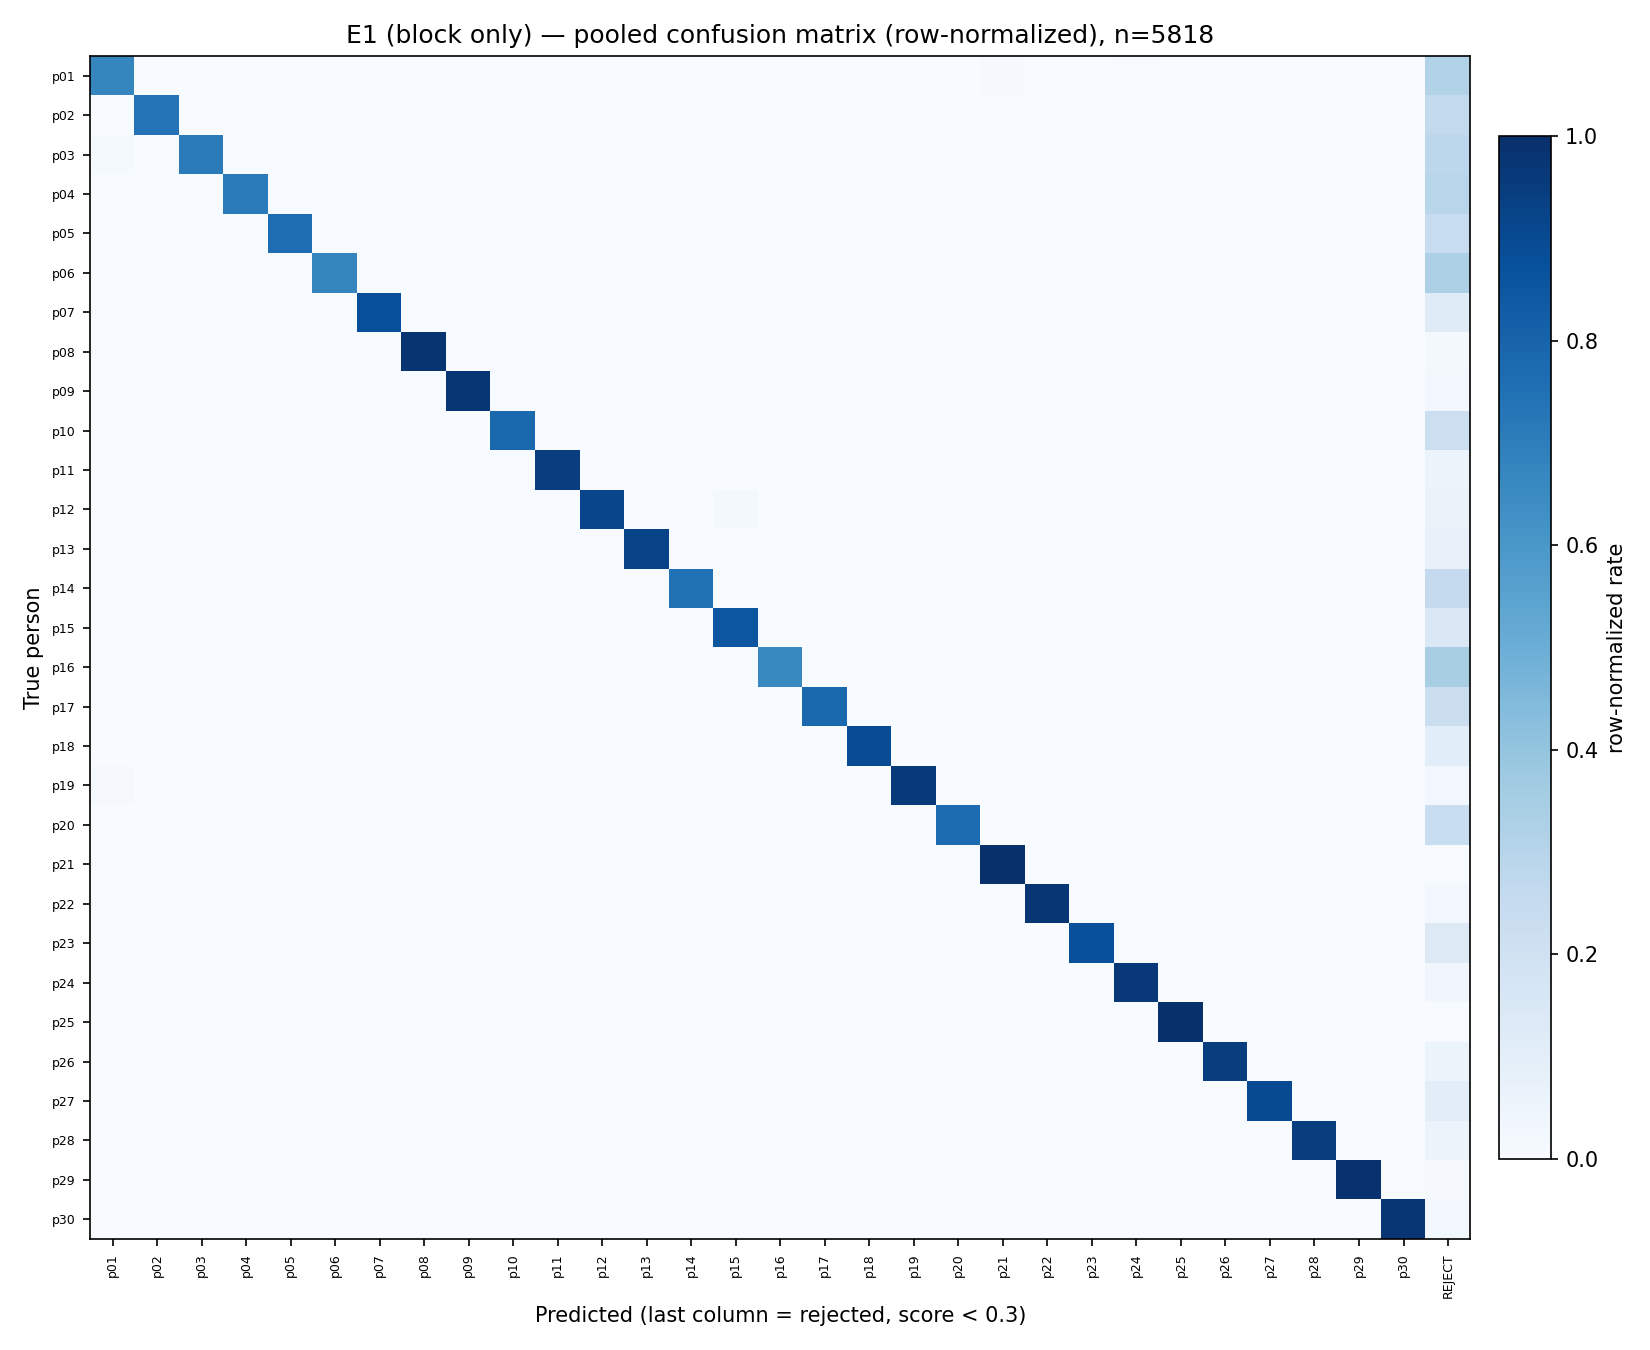
\includegraphics[width=\linewidth]{e1_confusion_overall.png}\caption{E1}
\end{subfigure}\hfill
\begin{subfigure}{.32\linewidth}\centering
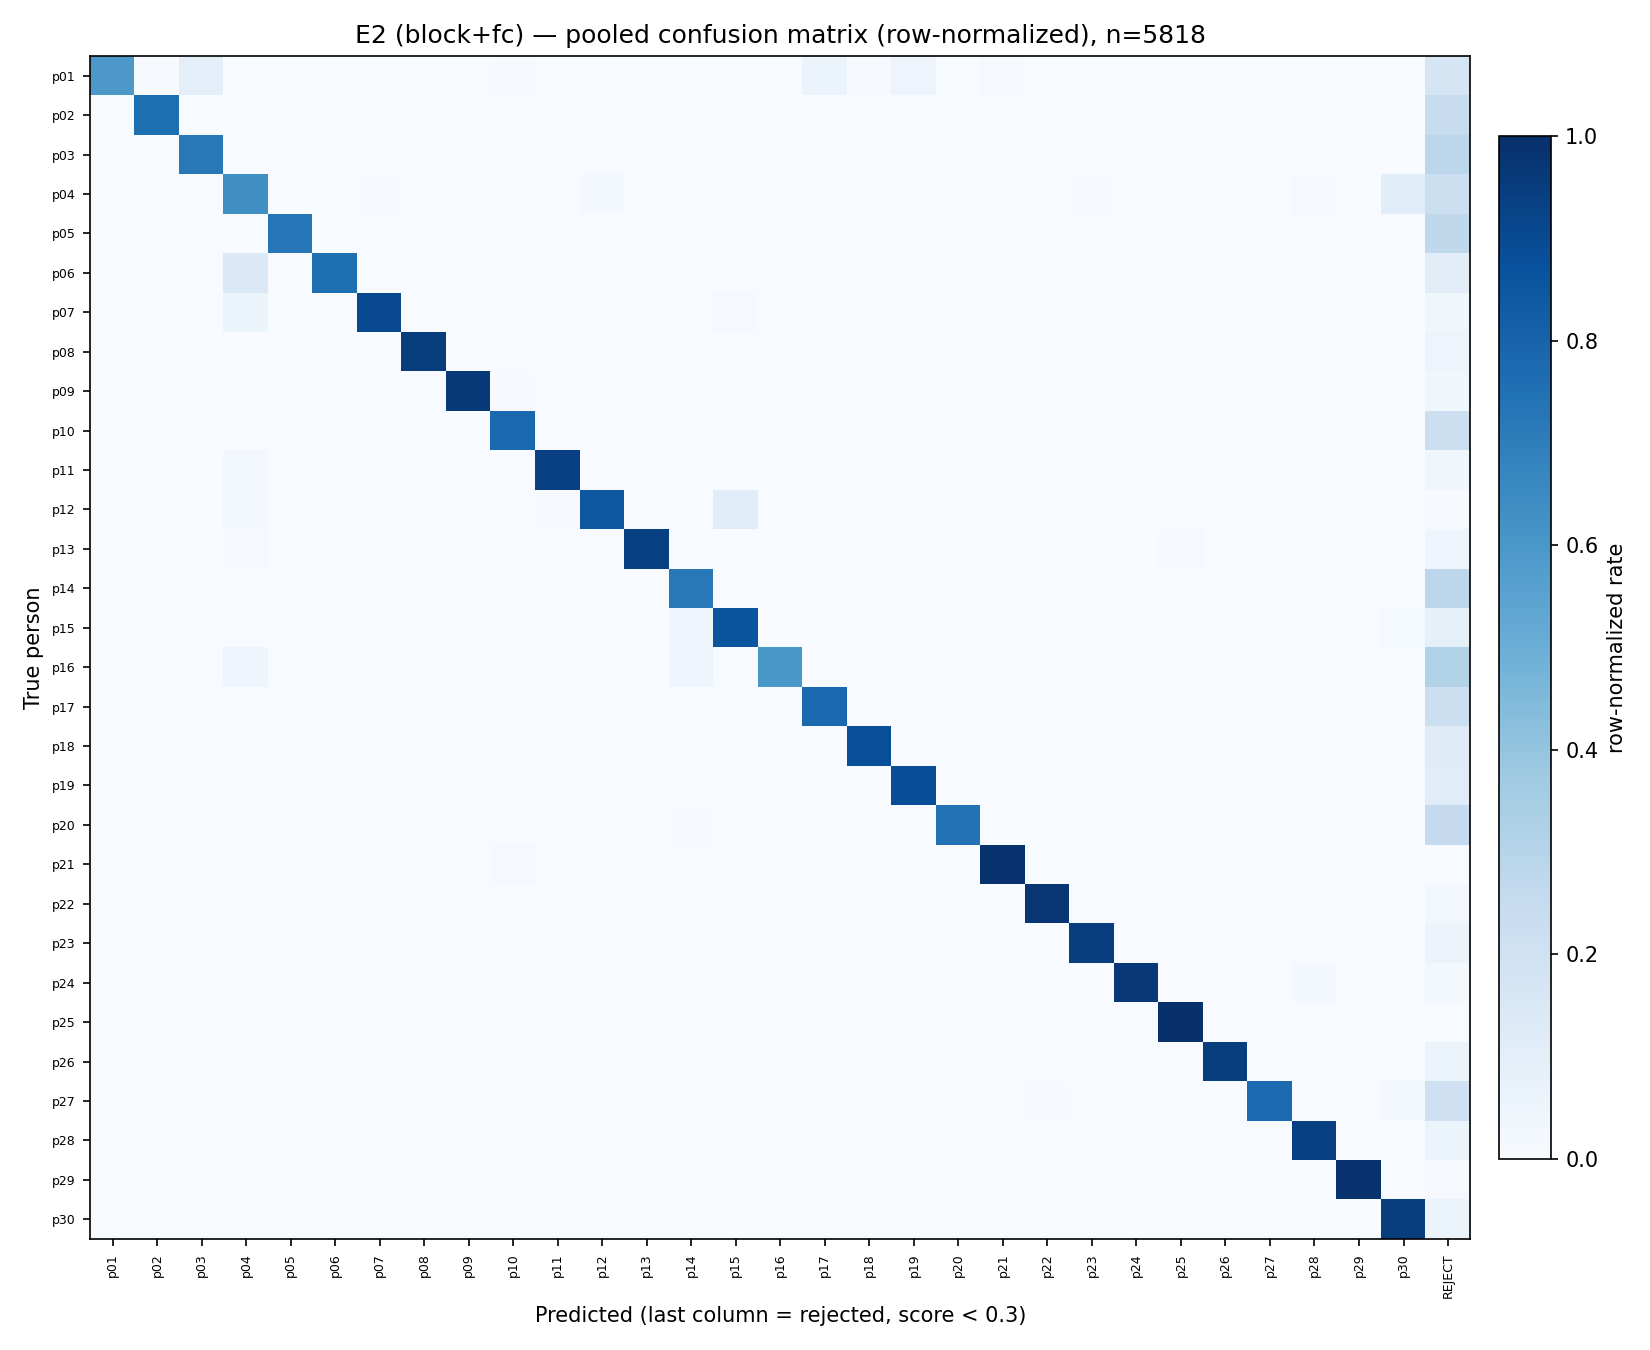
\includegraphics[width=\linewidth]{e2_confusion_overall.png}\caption{E2}
\end{subfigure}
\caption{Pooled 30-person confusion matrices with an additional \textsc{reject} output.}
\end{figure}

Precision stays high because wrong-person matches are rare; most lost recall appears in the reject column. E2's lower macro precision is the matrix-level expression of its 3.32\pct confident misidentification rate.

\section{Discussion and conclusion}

\begin{tcolorbox}[colback=traingreen!24,colframe=deepgreen,arc=4mm,boxrule=1pt,
  title={\textbf{Overall ranking: E1 $>$ E0 $>$ E2}}]
Only the narrow fine-tuning scope improves unseen-identity generalization reliably. E1 gains 1.20 percentage points pooled and wins in all six folds, while E2 is less accurate than the frozen baseline and produces more confident wrong-person matches.
\end{tcolorbox}

The architectural explanation is consistent with the measurements. E2 has 3.7 times more trainable parameters than E1, including a 12.85M-parameter matrix that directly redefines the 512-dimensional embedding space. Fitting that capacity using only 20 identities is disruptive and prone to identity-specific overfitting; the person-disjoint evaluation is specifically designed to expose that failure.

The benefit of E1 is also narrow: it is concentrated in \code{mask\_sunglass}, the only condition that simultaneously removes most information from both the upper and lower face. For milder conditions, the frozen ArcFace representation is already close to its practical ceiling and fine-tuning has little room to help.

\textbf{Practical recommendation.} For this enrollment scenario, retain the pretrained model unless double occlusion is an important operating condition. If fine-tuning is required, restrict it to the last residual block, preserve frozen BatchNorm statistics, retain epoch-0 fallback, and monitor confident misidentification separately from headline accuracy.

\section{Reproduction and file index}

All runs use seed 42. The pipeline can be reproduced in the following order.

\begin{lstlisting}[language=bash,caption={End-to-end reproduction commands.}]
# 1. Construct folds and select fold-independent benchmarks
python scripts/20_e1e2_person_folds.py

# 2. Train/evaluate E0, E1, and E2 over all folds
for fold in 1 2 3 4 5 6; do
  for exp in e0 e1 e2; do
    epochs_flag="--epochs 20"
    [ "$exp" = "e0" ] && epochs_flag="--epochs 0"
    python scripts/19_e1e2_person_finetune.py --exp $exp $epochs_flag \
      --setup metadata/e1e2_person_folds.json --fold $fold \
      --out-dir runs/e1e2/folds --accept-threshold 0.3
  done
done

# 3. Rebuild confusion matrices and per-image predictions
python scripts/21_e1e2_confusion.py --exp e0
python scripts/21_e1e2_confusion.py --exp e1
python scripts/21_e1e2_confusion.py --exp e2
python scripts/23_dump_predictions.py --exp e0
python scripts/23_dump_predictions.py --exp e1
python scripts/23_dump_predictions.py --exp e2

# 4. Reproduce the learning curves with validation loss
for fold in 1 2 3 4 5 6; do
  for exp in e1 e2; do
    python scripts/25_e1e2_learning_curve.py --exp $exp --epochs 20 \
      --setup metadata/e1e2_person_folds.json --fold $fold \
      --out-dir runs/e1e2/learning_curve --accept-threshold 0.3
  done
done

# 5. Generate all report plots
python scripts/22_e1e2_plots.py
python scripts/24_report_figures.py
\end{lstlisting}

\begin{longtable}{>{\raggedright\arraybackslash}p{.43\linewidth}>{\raggedright\arraybackslash}p{.51\linewidth}}
\caption{Project artefacts and their roles.}\\
\toprule
\textbf{Path} & \textbf{Contents}\\
\midrule
\endfirsthead
\toprule
\textbf{Path} & \textbf{Contents}\\
\midrule
\endhead
\code{metadata/manifest.csv} & Crop metadata: person, occlusion, lighting, detection score, and group ID.\\
\code{metadata/e1e2\_person\_folds.json} & Six fold assignments, benchmarks, and query exclusions.\\
\code{runs/e1e2/person\_benchmarks.npz} & Thirty fold-independent gallery embeddings.\\
\code{runs/e1e2/folds/fold\{1--6\}/} & E0/E1/E2 checkpoints, histories, and exact test results.\\
\code{runs/e1e2/learning\_curve/fold\{1--6\}/} & Reproduced histories with validation loss.\\
\code{runs/e1e2/analysis/*\_metrics.json} & Pooled confusion-derived metrics.\\
\code{runs/e1e2/analysis/*\_confusion*.csv} & Overall and per-occlusion confusion matrices.\\
\path{runs/e1e2/analysis/*_predictions.csv} & Per-image true identity, prediction, score, and outcome.\\
\code{docs/plots/*.png} & Raster figures embedded in this report.\\
\code{models/w600k\_r50.onnx} & ArcFace IResNet-50 recognizer.\\
\code{models/det\_10g.onnx} & SCRFD/RetinaFace-family detector.\\
\code{crops/} & All 5,988 aligned face crops.\\
\bottomrule
\end{longtable}

Companion sources are \code{report.md}, \code{confusion\_matrices.md}, and \code{epoch\_curves.md}. The present document consolidates their aggregate findings and adds publication-ready architecture and workflow figures.

\end{document}
